\documentclass[tikz,border=6pt]{standalone}
% Shared visual language for the book's standalone vector figures.
% Keep this file compatible with the TeX Live version used by LyX.
\usepackage{amsmath,amssymb}
\usepackage{array,booktabs}
\usepackage{pgfplots}
\usepackage{pgfplotstable}
\usetikzlibrary{arrows.meta,calc,positioning}
\pgfplotsset{compat=1.17}

\definecolor{BookBlue}{HTML}{0072B2}
\definecolor{BookOrange}{HTML}{D55E00}
\definecolor{BookGreen}{HTML}{009E73}
\definecolor{BookGray}{HTML}{666666}
\definecolor{BookLightGray}{HTML}{D9D9D9}

\pgfplotsset{
  book axis/.style={
    axis line style={black!75,line width=0.55pt},
    tick style={black!75,line width=0.45pt},
    tick label style={font=\small},
    label style={font=\small},
    legend style={
      font=\small,
      draw=none,
      fill=none,
      cells={anchor=west},
    },
    grid style={BookLightGray,line width=0.35pt},
    major grid style={BookLightGray,line width=0.35pt},
  },
}

\usepgfplotslibrary{groupplots}
\begin{document}
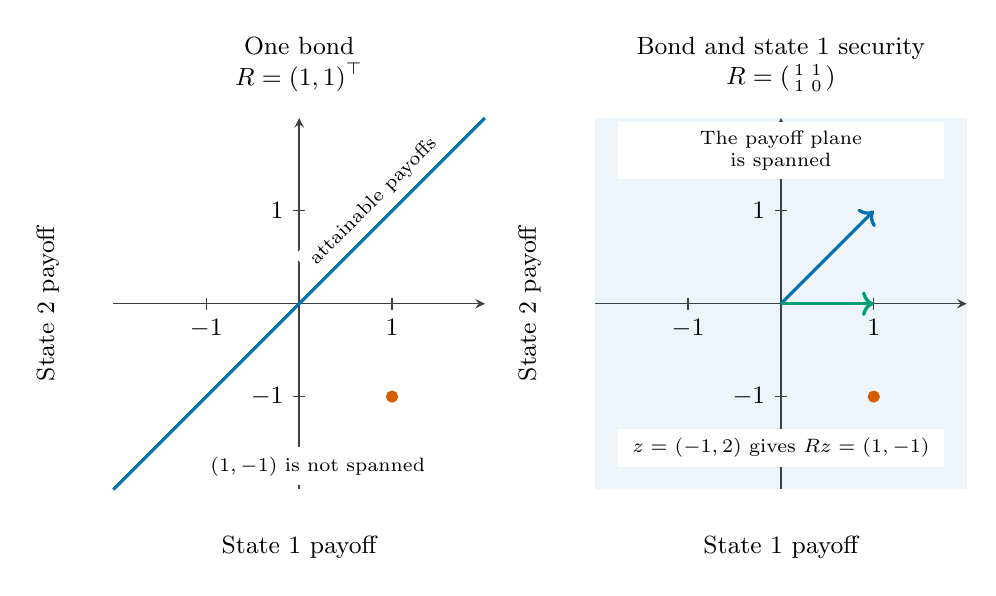
\begin{tikzpicture}
\begin{groupplot}[group style={group size=2 by 1,horizontal sep=1.4cm},book axis,
 width=6.3cm,height=6.3cm,xmin=-2,xmax=2,ymin=-2,ymax=2,
 axis lines=middle,xtick={-1,1},ytick={-1,1},xlabel={State 1 payoff},ylabel={State 2 payoff},
 label style={font=\small},title style={font=\small,align=center},
 xlabel style={at={(axis description cs:.5,-.10)},anchor=north},
 ylabel style={at={(axis description cs:-.12,.5)},anchor=south,rotate=90},
 clip=false]
 \nextgroupplot[title={One bond\\$R=(1,1)^{\top}$}]
 \addplot[BookBlue,very thick,domain=-2:2]{x};
 \addplot[only marks,mark=*,mark size=2pt,BookOrange] coordinates{(1,-1)};
 \node[font=\scriptsize,fill=white,align=center,text width=3.1cm]
   at(axis cs:.2,-1.75){$(1,-1)$ is not spanned};
 \node[font=\scriptsize,rotate=45,fill=white]
   at(axis cs:.8,1.1){attainable payoffs};
 \nextgroupplot[title={Bond and state 1 security\\$R=\left(\begin{smallmatrix}1&1\\1&0\end{smallmatrix}\right)$},
   axis background/.style={fill=BookBlue!7}]
 \draw[->,BookBlue,very thick] (axis cs:0,0)--(axis cs:1,1);
 \draw[->,BookGreen,very thick] (axis cs:0,0)--(axis cs:1,0);
 \addplot[only marks,mark=*,mark size=2pt,BookOrange] coordinates{(1,-1)};
 \node[font=\scriptsize,fill=white,align=center,text width=3.9cm]
   at(axis cs:0,-1.55){$z=(-1,2)$ gives $Rz=(1,-1)$};
 \node[font=\scriptsize,fill=white,align=center,text width=3.9cm]
   at(axis cs:0,1.65){The payoff plane\\is spanned};
\end{groupplot}
\end{tikzpicture}
\end{document}
